\section{Overview of our Approach}\label{sec:overview}
Figure \ref{flow} presents the overview of our approach \tool, which consists of three components. Taking a satisfiable formula
$\Phi$ as an input, \tool first computes an under-approximation $\NBLap(\Phi)\subseteq \NBL(\Phi)$ of the non-backbone of
$\Phi$. Then, \tool computes an approximation $\BLap(\Phi)$ of the backbone of $\Phi$ based on the set $\NBLap(\Phi)$, where each literal $l\in \BLap(\Phi)$ has a high possibility to be a backbone literal of $\Phi$.
Finally, \tool removes non-backbone literals from $\BLap(\Phi)$ and adds backbone literals into $\BLap(\Phi)$ to compute the exact backbone of $\Phi$.
\begin{figure*}[t]
   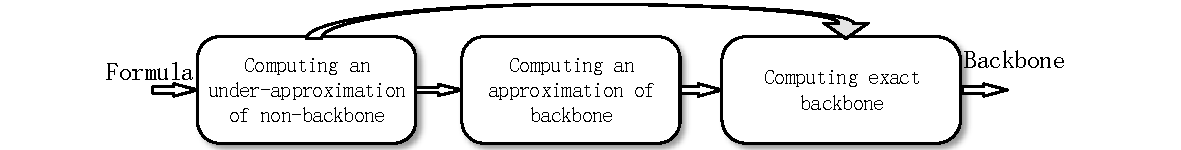
\includegraphics[scale=0.75]{Framework}
  \hspace*{30mm} 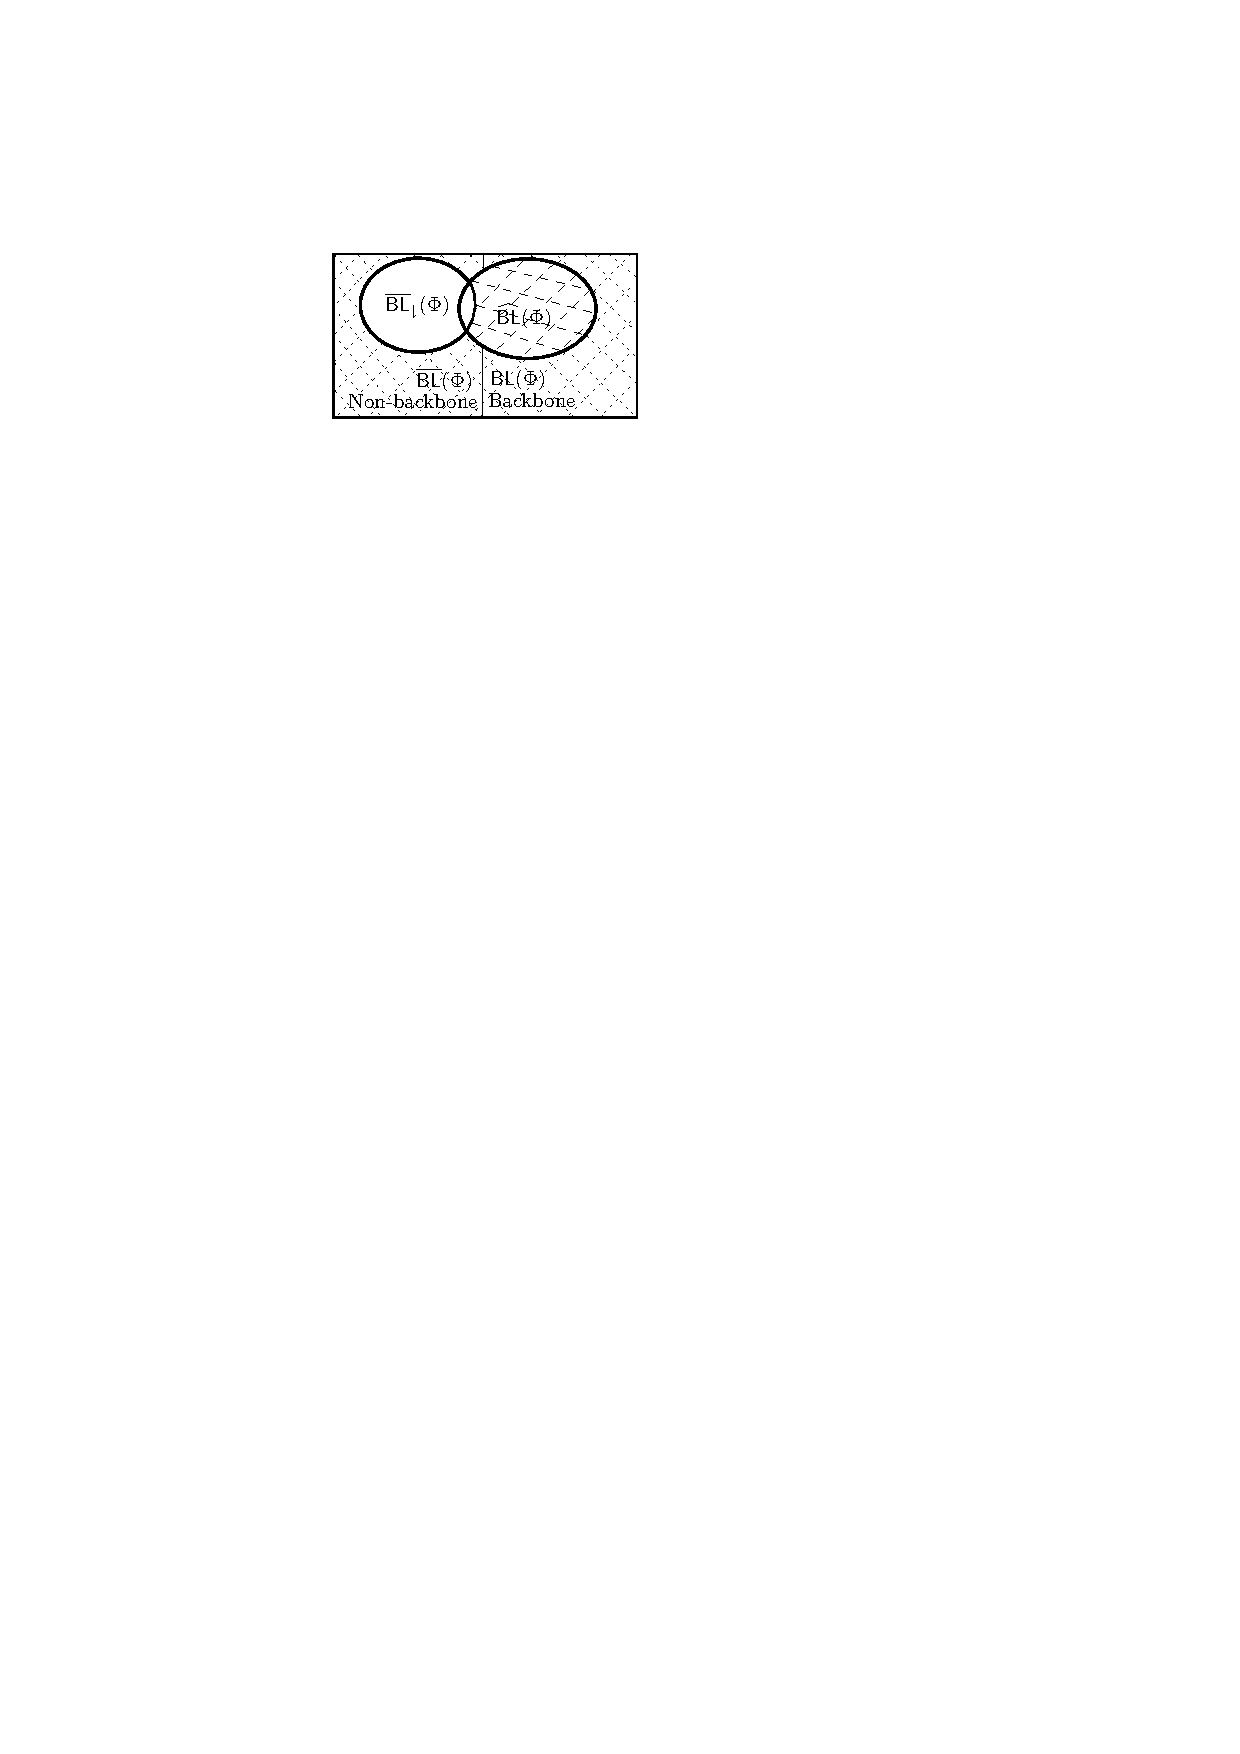
\includegraphics[scale=0.75]{Fig-backbone}
   \caption{Overview of our approach}
   \label{flow}
\end{figure*}

As shown in Figure \ref{flow}, $\NBLap(\Phi)$ only contains a part of non-backbone literals.
Most of the literals in $\BLap(\Phi)$ are backbone, only a small part of them is non-backbone.
In iterative testing (step 3), experiments show that solving time are saved by testing the literals in $\BLap(\Phi)$ first. It's because that there is a higher possibility to choose a backbone from $\BLap(\Phi)$. With more known backbone literals, SAT testings are accelerated.

\medskip
\noindent{\bf Computing an under-approximation of non-backbone.}
Given a satisfiable formula $\Phi$, we first compute a model $\lambda$ of $\Phi$ by calling a SAT solver.
From the model $\lambda$, we compute a base under-approximation of non-backbone.
Later, we apply a Greedy-based algorithm to add more non-backbone literals into the base set, which results in $\NBLap(\Phi)$.

The algorithm iteratively computes new models based on the original model $\lambda$, by changing exactly one literal at each iteration. Suppose there are k iterations in Greedy-based Algorithm, then k new models will be generated. New non-backbone are found from each new model. The heuristic strategy for Greedy-based algorithm is changing the literal that satisfies the least clauses at each iteration. When changing a literal's assignment, clauses remain their satisfiability if this literal is not their satisfied litera. Choosing the literal that satisfies the least clauses will affects the least clauses, which lead to a higher possibility of finding a new model.

\medskip
\noindent{\bf Computing an approximation of backbone.}
At this step, we apply a Whitening-based algorithm to compute the approximation $\BLap(\Phi)$.
Whitening Algorithm was used to compute \emph{essential node}, that are nodes can't be colored as white without changing the color of its adjacent nodes in a graph coloring problem.


We consider essential nodes as backbone literals in backbone computing.
To increase the proportion of backbone literals found by Whitening Algorithm, we use two heuristic strategies to refine Whitening Algorithm.
First, we check whether the generated assignment is a model to eliminate some of the non-backbone literals returned by Whitening-based Algorithm.
Moreover, we use assumptions features of MINISAT \cite{JLM15} to find some accurate backbone literals.
With the refinement of heuristic strategies, Whitening-based Algorithm is able to return a set of literals that are highly likely to be backbone.


\medskip
\noindent{\bf Computing exact backbone.}
At this step, we use Algorithm 3 (Iterative Algorithm) from \cite{JLM15} to compute backbone.
This algorithm uses SAT solvers to test whether a literal is a backbone literal or not.
For instance, if $\Phi\wedge \neg l$ is unsatisfiable but $\Phi$ is satisfiable, then $l$ must be a backbone literal of $\Phi$.

We first iteratively select one literal $l$ from $\BLap(\Phi)\setminus \NBLap(\Phi)$ such that $\lambda \models \neg l$ and test $l$ by checking the satisfiability of $\Phi\wedge l$ (dashed area in Figure \ref{flow}).
If $l$ is a backbone, we will add $l$ into $\Phi$ as a clause. Adding known backbone literals into $\Phi$ as clauses potentially speedups the later SAT testing \cite{JLM15,MPA2015}.
Then, we do the same testing for literals from $\Lit(\Phi)\setminus (\NBLap(\Phi)\cup\BLap(\Phi))$ (dotted area in Figure \ref{flow}).
After this step, the exact backbone and non-backbone are found.


In general, one can directly test all the literals to compute backbone without the two approximations.
However, the test heavily relies on SAT solving which may be time-cost.
Our approach makes two contributions compared to this na\"{\i}ve approach.
One is that we reduce the number of SAT calls using the known non-backbone literals $\BLap(\Phi)$.
The another one is that we first check literals that have high probability to be backbone literals so that backbone literals can be found as early as possible.


